% 
% https://pgfplots.net/multi-series-bar-chart/
% https://pgfplots.net/stacked-bar-plot/
% https://tex.stackexchange.com/questions/131349/clustered-stacked-bar-chart-overlapping-labels
\documentclass[varwidth=12cm,border=1cm,tikz]{standalone}
\usepackage[ipaex]{luatexja-preset} % standaloneとlualatexjaを共存させる方法?
\usepackage{tikz, pgf, pgfplots, pgfplotstable}
\usepackage{physics}
\pgfplotsset{compat = newest}
\usepackage{tikz-3dplot}
\usepackage{xcolor}

%\usepackage[style=phys,backend=bibtex]{biblatex}
\usetikzlibrary{math,calc,patterns}
\usepgfplotslibrary{groupplots} % LATEX and plain TEX
% \usepackage[numbers]{natbib}
\usepackage[square, numbers, sort&compress]{natbib}
% revtex4-2 は natbib を中で usepackage している
% square : [] で囲む
% numbers : 通し番号で表現
% sort&compress : 連続する文献はハイフンでつなぐ
\bibliographystyle{apsrev4-1} % MacTex なら入ってると思うが必要なら CTAN から引っ張ってくる

\usepackage{siunitx}
%\setcitestyle{numbers,open={((},close={))}} %Citation-related commands

% axis style, ticks, etc
\pgfplotsset{every axis/.append style={
                    label style={font=\Huge}, % ラベルだけ大きく
		    title style={font=\huge},
                    tick label style={font=\huge},
		    legend style={font=\huge},
                   }}
\usepgfplotslibrary{colorbrewer}
\usetikzlibrary{pgfplots.colorbrewer}
\usetikzlibrary{arrows.meta,backgrounds}
\tikzset{white background/.style={show background rectangle,tight background,background rectangle/.style={fill=white}}}

% %https://tex.stackexchange.com/questions/13627/pgfplots-multiple-shifted-stacked-plots-in-one-diagram
 \makeatletter
  \newcommand\resetstackedplots{
  \makeatletter
  \pgfplots@stacked@isfirstplottrue
  \makeatother
  \addplot [forget plot,draw=none] coordinates{(1,0) (2,0) (3,0) (4,0)};
  }
 \makeatother


\begin{document} 
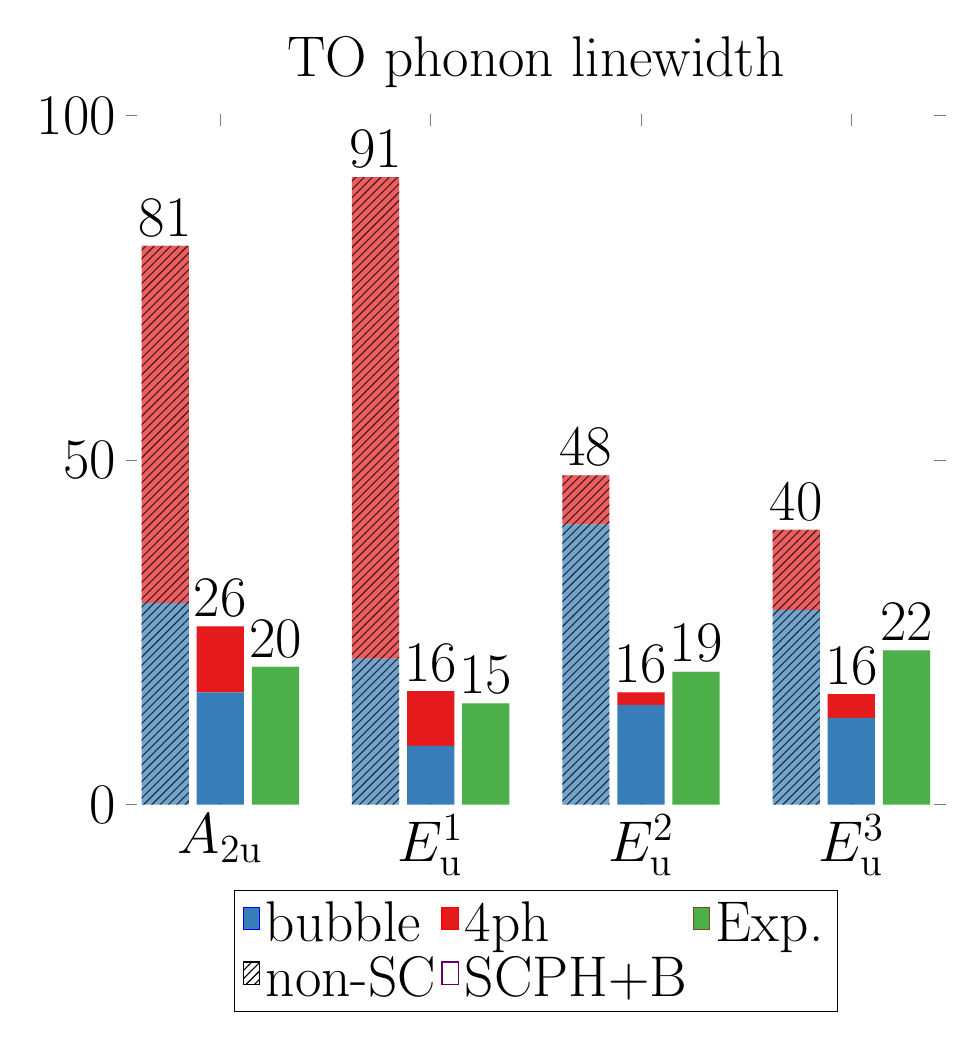
\begin{tikzpicture}[white background]
\begin{axis}[ 
   ybar stacked, % ybar (通常のbar plot) 
% nodes near coords style={/pgf/number format/.cd,precision=1}
%nodes near coords style={/pgf/number format/.cd,precision=1},
   xtick={1,2,3,4},
% https://bvieuble.github.io/projects/6_texfty/
%   nodes near coords,% (値をprintする場合)
%   every node near coord/.append style={font=\normalsize,above},
   ytick distance = 50,
   width = 12cm, 
   bar width=0.6cm,
   title=TO phonon linewidth,
   xticklabels={$A_{\mathrm{2u}}$,$E^{1}_{\mathrm{u}}$,$E^{2}_{\mathrm{u}}$,$E^{3}_{\mathrm{u}}$},
%   /pgf/number format/1000 sep={}, 
   y axis line style={opacity=0},
%   axis y line*=none,
 %  axis x line*=none,
   ymin=0,
   % xtick=data,
   enlarge x limits=0.15,
   %symbolic x coords={
   %        $A_{\mathrm{2u}}$, $E^{1}_{\mathrm{u}}$, $E^{2}_{\mathrm{u}}$, $E^{3}_{\mathrm{u}}$},
   legend style={ at={(0.5,-0.3)},anchor=south,legend columns=-1 } ,
   legend cell align = {left},
   % legend pos = north east,
%   transpose legend,
   legend columns=3,
  ] 
% 実験値
%    $E^{1}_{\mathrm{u}}$        &$21.2$ & $69.9$ & $91.1$ && $8.54$  & $7.95$  & $16.4$  &&  $14.7\pm 8.0$  \\
%    $E^{2}_{\mathrm{u}}$        &$40.7$ & $7.09$ & $47.8$ && $14.5$  & $1.81$  & $16.2$  &&  $19.3\pm 2.8$  \\
%    $E^{3}_{\mathrm{u}}$        &$28.3$ & $11.6$ & $39.9$ && $12.6$  & $3.47$  & $16.0$  &&  $22.4\pm 3.1$  \\
%    $A_{\mathrm{2u}}$           &$29.3$ & $51.8$ & $81.1$ && $16.3$  & $9.57$  & $25.7$  &&  $20.0\pm 10.2$ \\
%
% \addplot+ coordinates {};
%% >>>> NON-SC >>>>> 
% https://tex.stackexchange.com/questions/24964/how-to-combine-fill-and-pattern-in-a-pgfplot-bar-plot
 \addplot+ [bar shift=-0.7cm, fill=Set1-B, draw=none, opacity=0.7, forget plot, postaction={pattern=north east lines}] coordinates { 
                                          (1, 29.3) 
                                          (2, 21.2)
                                          (3, 40.7)
                                          (4, 28.3)}; % non-SC bubble

 \addplot+ [bar shift=-0.7cm, fill=Set1-A, draw=none, opacity=0.7, forget plot, postaction={pattern=north east lines}] coordinates { 
                                          (1, 51.8) 
                                          (2, 69.9)
                                          (3, 7.09)
                                          (4, 11.6)}; % non-SC 4ph

 % \addplot+ [bar shift=-0.7cm, fill=Set1-C, draw=none] coordinates { (1,0) 
 %                                          (2, 0)
 %                                          (3, 0)
 %                                          (4, 0)}; % for legend(dummy)

% for topper (non-SC)
%https://tex.stackexchange.com/questions/411600/pgfplot-tikz-stacked-bar-chart-with-compat-1-9-or-later
  \addplot+ [nodes near coords,point meta=y,nodes near coords style={anchor=south,color=black,font=\huge,/pgf/number format/.cd,precision=0},bar shift=-0.7cm, fill=Set1-A,draw=none,forget plot] coordinates { 
                                          (1, 0.001) 
                                          (2, 0.001)
                                          (3, 0.001)
                                          (4, 0.001)}; 


%\addplot+ coordinates { (1, 12) (2, 11) };
%\addplot+ coordinates { (1, 54) (2, 50) };

% \addplot+ coordinates { (A2u, 34) (E1u, 39) (2012, 39) (2013, 36) (2014, 32.6) }; 
%\addplot+ coordinates { (A2u, 12) (E1u, 11) (2012, 14) (2013, 12) (2014, 10.7) }; 
%\addplot+ coordinates { (A2u, 54) (E1u, 50) (2012, 47) (2013, 52) (2014, 56.7) }; 

\resetstackedplots
 \addplot+ [fill=Set1-B,draw=none] coordinates {    (1, 16.3) 
                                          (2, 8.54)
                                          (3, 14.5)
                                          (4, 12.6)}; % SCPH+B bubble
 \addplot+ [fill=Set1-A,draw=none] coordinates {    (1, 9.57) 
                                          (2, 7.95)
                                          (3, 1.81)
                                          (4, 3.47)}; % SCPH+B 4ph

% for topper (SCPH+B)
%https://tex.stackexchange.com/questions/411600/pgfplot-tikz-stacked-bar-chart-with-compat-1-9-or-later
  \addplot+ [nodes near coords,point meta=y,nodes near coords style={anchor=south,color=black,font=\huge,/pgf/number format/.cd,precision=0},fill=Set1-A,draw=none,forget plot] coordinates { 
                                          (1, 0.001) 
                                          (2, 0.001)
                                          (3, 0.001)
                                          (4, 0.001)}; % non-SC 4ph


\resetstackedplots
 \addplot+ [bar shift=.7cm,fill=Set1-C,draw=none] coordinates { (1, 20.0) 
                                          (2, 14.7)
                                          (3, 19.3)
                                          (4, 22.4)}; % Exp.

% for topper (Exp.)
%https://tex.stackexchange.com/questions/411600/pgfplot-tikz-stacked-bar-chart-with-compat-1-9-or-later
  \addplot+ [nodes near coords,point meta=y,nodes near coords style={anchor=south,color=black,font=\huge,/pgf/number format/.cd,precision=0},bar shift=.7cm,fill=Set1-C,draw=none,forget plot] coordinates { 
                                          (1, 0.001) 
                                          (2, 0.001)
                                          (3, 0.001)
                                          (4, 0.001)}; % Exp


% total value
% \node[font=\large,anchor=south] at (0.8,91.1)  {$91.1$};
% \node[font=\large,anchor=south] at (0.78,81.1)  {$81.1$};

% \node[] at (axis cs:5,190)  {$91.1$};

% legend for non-SC vs SCPH+B
  \addplot+ [pattern=north east lines] coordinates { 
                                          (1, 0.0) 
                                          (2, 0.0)
                                          (3, 0.0)
                                          (4, 0.0)}; %


  \addplot+ [fill=white] coordinates { 
                                          (1, 0.0) 
                                          (2, 0.0)
                                          (3, 0.0)
                                          (4, 0.0)}; %


\legend{bubble,4ph,Exp., non-SC, SCPH+B}

\end{axis} 
\end{tikzpicture} 
\end{document}


